\chapter{Results and Evaluation}
\label{ch:results}
The main in goal of this thesis was to analyze the relation between force, area and position of the presented FSR and create a data fitting routines to estimate contact size, exerted force and position. In this chapter the results of the thesis are presented and its accuracy evaluated.


\section{Measurements}



\subsection{Position}

One task of the thesis was to evaluate accuracy of the given FSR and identify whether it was possible to set up a sensor system detecting position within sub millimeter range.

\begin{figure}%
    \centering
    \subfloat[Raw]{{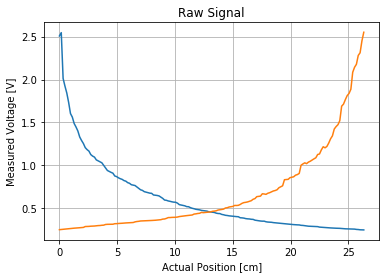
\includegraphics[width=5cm]{images./Positionraw.png}} }
    \label{fig:rawpos}
    \qquad
    \subfloat[Converted]{{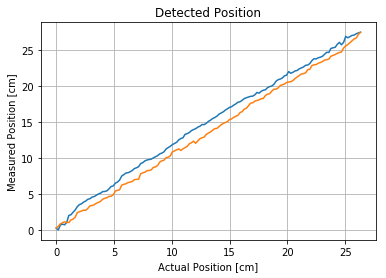
\includegraphics[width=5cm]{images./Position.png}} }
    \caption{2 Figures side by side}%
    \label{fig:positions}%
\end{figure}

\subsection{Area vs Force}

\begin{figure}[htp]
    \centering
    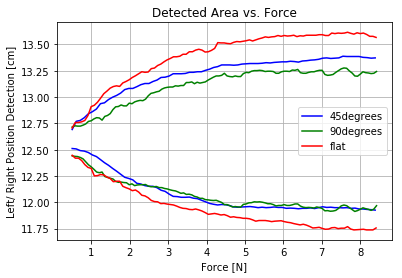
\includegraphics[width=10cm]{images./ForcevsArea.png}
    \caption[Area Detection]{Exerted Force }
    \label{fig:operatingmode}
\end{figure}  

\subsection{Accuracy}




As mentioned in \ref{subsection:accuracy} deviation \todo{graph with deviation}

